\documentclass{standalone}
\usepackage{graphicx}	
\usepackage{amssymb, amsmath}
\usepackage{color}

\usepackage{tikz}
\usetikzlibrary{calc, arrows.meta}
\usepackage{pgfmath}

\definecolor{light}{RGB}{220, 188, 188}
\definecolor{mid}{RGB}{185, 124, 124}
\definecolor{dark}{RGB}{143, 39, 39}
\definecolor{highlight}{RGB}{180, 31, 180}
\definecolor{gray10}{gray}{0.1}
\definecolor{gray20}{gray}{0.2}
\definecolor{gray30}{gray}{0.3}
\definecolor{gray40}{gray}{0.4}
\definecolor{gray60}{gray}{0.6}
\definecolor{gray70}{gray}{0.7}
\definecolor{gray80}{gray}{0.8}
\definecolor{gray90}{gray}{0.9}
\definecolor{gray95}{gray}{0.95}

\newcommand*{\offset}{0.025}

\begin{document}

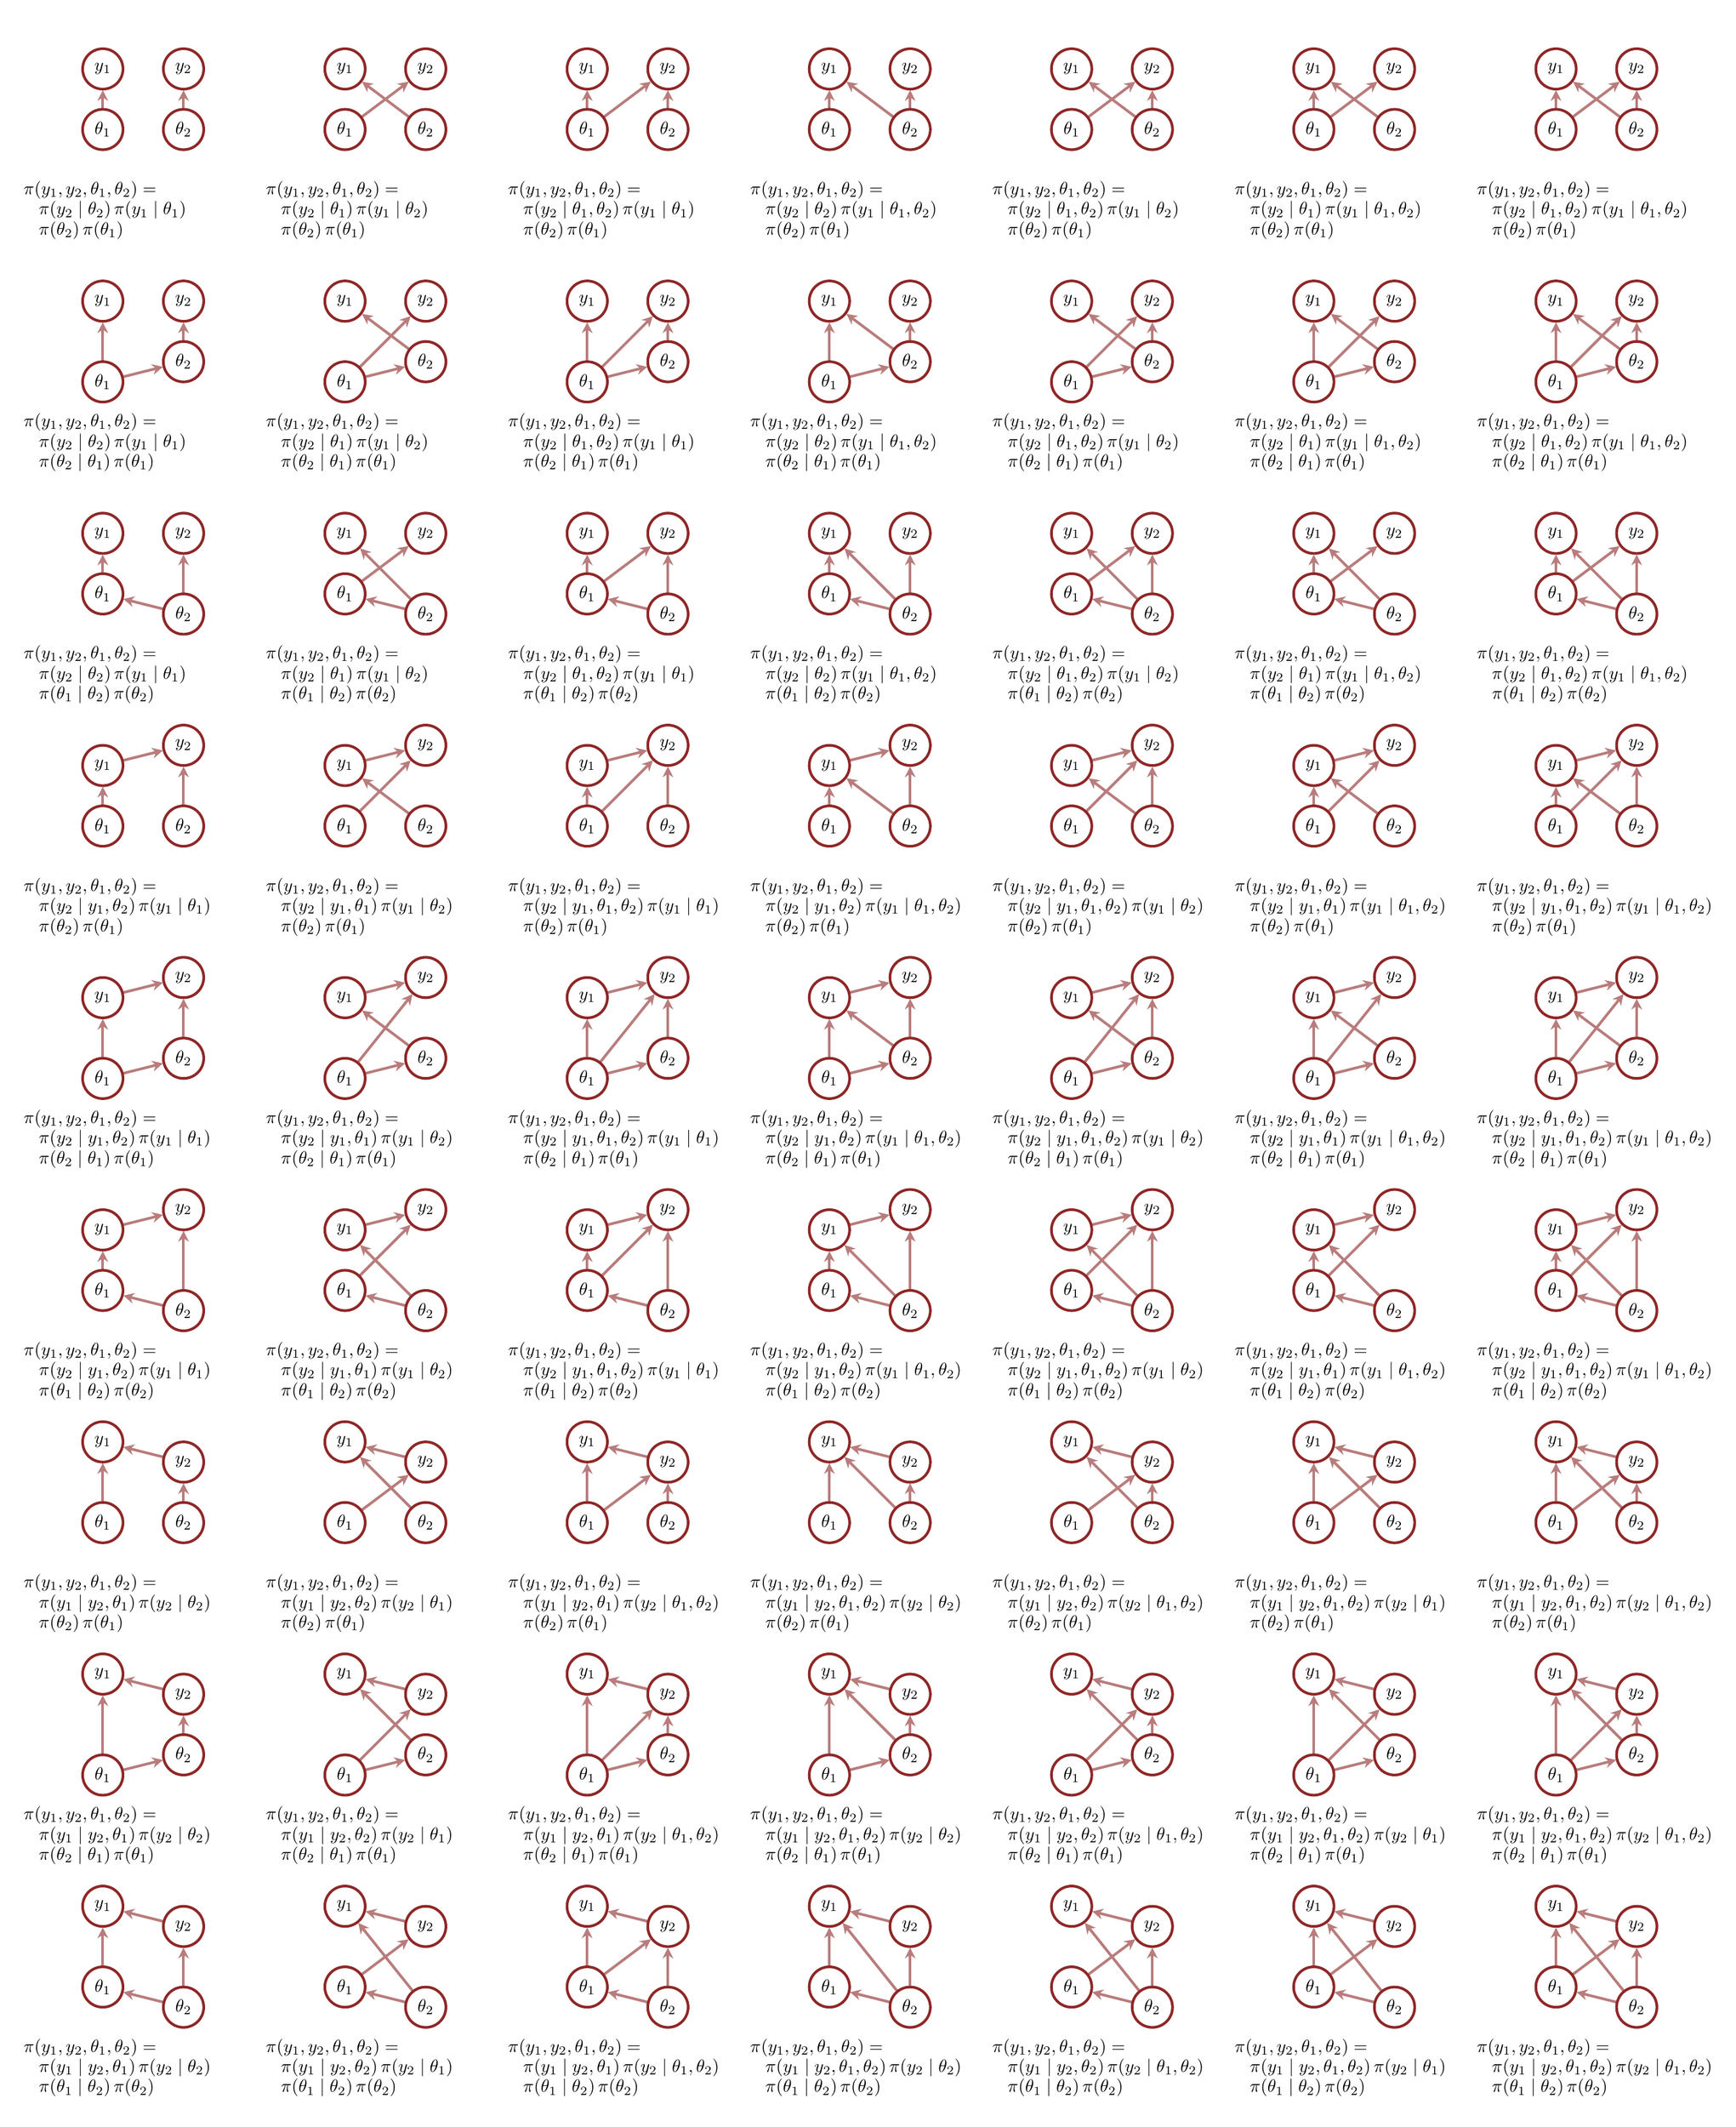
\begin{tikzpicture}[scale=0.2, thick]

\pgfmathsetmacro{\r}{2}


\foreach \n in {0, 1, ..., 62} {

  \pgfmathtruncatemacro{\i}{mod(\n, 7)}
  \pgfmathtruncatemacro{\j}{mod(floor(\n / 7), 3)}
  \pgfmathtruncatemacro{\k}{floor(floor(\n / 7) / 3)}
  \pgfmathsetmacro{\dx}{24 * mod(\n, 7)}
  \pgfmathsetmacro{\dy}{-23 * floor(\n / 7)}

  \begin{scope}[shift={(\dx, \dy)}]
    \draw[white] (-12, -15) rectangle (12, 8);

    \ifnum\j=0 
      \coordinate (A) at (-4, -3);
      \coordinate (B) at (+4, -3);
      \def\a{\theta_{1}}
      \def\conda{}
      \def\b{\theta_{2}}
      \def\condb{}
    \fi 
    
    \ifnum\j=1
      \coordinate (A) at (-4, -5);
      \coordinate (B) at (+4, -3);
      \draw[-{Stealth[length=6pt, width=6pt]}, shorten >=12, color=mid, line width=1.5] (A) -- (B);
      \def\a{\theta_{1}}
      \def\conda{}
      \def\b{\theta_{2}}
      \def\condb{\mid \theta_{1}}
    \fi
    
    \ifnum\j=2
      \coordinate (A) at (-4, -3);
      \coordinate (B) at (+4, -5);
      \draw[-{Stealth[length=6pt, width=6pt]}, shorten >=12, color=mid, line width=1.5] (B) -- (A);
      \def\a{\theta_{2}}
      \def\conda{}
      \def\b{\theta_{1}}
      \def\condb{\mid \theta_{2}}
    \fi

    \ifnum\k=0 
      \coordinate (C) at (-4, +3);
      \coordinate (D) at (+4, +3);
      \def\c{y_{1}}
      \def\condc{\mid}
      \def\d{y_{2}}
      \def\condd{\mid}
    \fi 
    
    \ifnum\k=1
      \coordinate (C) at (-4, +3);
      \coordinate (D) at (+4, +5);
      \draw[-{Stealth[length=6pt, width=6pt]}, shorten >=12, color=mid, line width=1.5] (C) -- (D);
      \def\c{y_{1}}
      \def\condc{\mid}
      \def\d{y_{2}}
      \def\condd{\mid y_{1}, }
    \fi 
    
    \ifnum\k=2
      \coordinate (C) at (-4, +5);
      \coordinate (D) at (+4, +3);
      \draw[-{Stealth[length=6pt, width=6pt]}, shorten >=12, color=mid, line width=1.5] (D) -- (C);
      \def\c{y_{2}}
      \def\condc{\mid}
      \def\d{y_{1}}
      \def\condd{\mid y_{2}, }
    \fi
    
    \ifnum\i=0 
      \draw[-{Stealth[length=6pt, width=6pt]}, shorten >=12, color=mid, line width=1.5] (A) -- (C);
      \draw[-{Stealth[length=6pt, width=6pt]}, shorten >=12, color=mid, line width=1.5] (B) -- (D);
      
      \ifnum\k=2
        \def\conddi{\condd \theta_{1}}
        \def\condci{\condc \theta_{2}}
      \else      
        \def\condci{\condc \theta_{1}}
        \def\conddi{\condd \theta_{2}}
      \fi
    \fi
   
    \ifnum\i=1
      \draw[-{Stealth[length=6pt, width=6pt]}, shorten >=12, color=mid, line width=1.5] (A) -- (D);
      \draw[-{Stealth[length=6pt, width=6pt]}, shorten >=12, color=mid, line width=1.5] (B) -- (C);
      
      \ifnum\k=2
        \def\conddi{\condd \theta_{2}}
        \def\condci{\condc \theta_{1}}
      \else  
        \def\condci{\condc \theta_{2}}
        \def\conddi{\condd \theta_{1}}    
      \fi
    \fi
      
    \ifnum\i=2
      \draw[-{Stealth[length=6pt, width=6pt]}, shorten >=12, color=mid, line width=1.5] (A) -- (C);
      \draw[-{Stealth[length=6pt, width=6pt]}, shorten >=12, color=mid, line width=1.5] (A) -- (D);
      \draw[-{Stealth[length=6pt, width=6pt]}, shorten >=12, color=mid, line width=1.5] (B) -- (D);
      
      \ifnum\k=2
        \def\conddi{\condd \theta_{1}}
        \def\condci{\condc \theta_{1}, \theta_{2}}
      \else 
        \def\condci{\condc \theta_{1}}
        \def\conddi{\condd \theta_{1}, \theta_{2}}     
      \fi
    \fi
      
    \ifnum\i=3
      \draw[-{Stealth[length=6pt, width=6pt]}, shorten >=12, color=mid, line width=1.5] (A) -- (C);
      \draw[-{Stealth[length=6pt, width=6pt]}, shorten >=12, color=mid, line width=1.5] (B) -- (C);
      \draw[-{Stealth[length=6pt, width=6pt]}, shorten >=12, color=mid, line width=1.5] (B) -- (D);
      
      \ifnum\k=2
        \def\conddi{\condd \theta_{1}, \theta_{2}}
        \def\condci{\condc \theta_{2}}
      \else      
        \def\condci{\condc \theta_{1}, \theta_{2}}
        \def\conddi{\condd \theta_{2}}
      \fi
    \fi
     
    \ifnum\i=4
      \draw[-{Stealth[length=6pt, width=6pt]}, shorten >=12, color=mid, line width=1.5] (A) -- (D);
      \draw[-{Stealth[length=6pt, width=6pt]}, shorten >=12, color=mid, line width=1.5] (B) -- (C);
      \draw[-{Stealth[length=6pt, width=6pt]}, shorten >=12, color=mid, line width=1.5] (B) -- (D);
      
      \ifnum\k=2
        \def\conddi{\condd \theta_{2}}
        \def\condci{\condc \theta_{1}, \theta_{2}}
      \else      
        \def\condci{\condc \theta_{2}}
        \def\conddi{\condd \theta_{1}, \theta_{2}}
      \fi
    \fi
     
    \ifnum\i=5
      \draw[-{Stealth[length=6pt, width=6pt]}, shorten >=12, color=mid, line width=1.5] (A) -- (C);
      \draw[-{Stealth[length=6pt, width=6pt]}, shorten >=12, color=mid, line width=1.5] (A) -- (D);
      \draw[-{Stealth[length=6pt, width=6pt]}, shorten >=12, color=mid, line width=1.5] (B) -- (C);
      
      \ifnum\k=2
        \def\conddi{\condd \theta_{1}, \theta_{2}}
        \def\condci{\condc \theta_{1}}
      \else      
        \def\condci{\condc \theta_{1}, \theta_{2}}
        \def\conddi{\condd \theta_{1}}
      \fi
    \fi
      
    \ifnum\i=6
      \draw[-{Stealth[length=6pt, width=6pt]}, shorten >=12, color=mid, line width=1.5] (A) -- (C);
      \draw[-{Stealth[length=6pt, width=6pt]}, shorten >=12, color=mid, line width=1.5] (A) -- (D);
      \draw[-{Stealth[length=6pt, width=6pt]}, shorten >=12, color=mid, line width=1.5] (B) -- (C);
      \draw[-{Stealth[length=6pt, width=6pt]}, shorten >=12, color=mid, line width=1.5] (B) -- (D);    
      
      \ifnum\k=2
        \def\conddi{\condd \theta_{1}, \theta_{2}}
        \def\condci{\condc \theta_{1}, \theta_{2}}
      \else  
        \def\condci{\condc \theta_{1}, \theta_{2}}
        \def\conddi{\condd \theta_{1}, \theta_{2}}    
      \fi
    \fi
    
    \node[anchor=west] at (-12.5, -9) { $\pi(y_{1}, y_{2}, \theta_{1}, \theta_{2}) =$ };
    \node[anchor=west] at (-11, -11) { $\pi(\d \conddi) \, \pi(\c \condci)$ };
    \node[anchor=west] at (-11, -13) { $\pi(\b \condb) \, \pi(\a \conda)$ };

    \filldraw[fill=white, draw=dark, line width=1.5] (A) circle (\r)
    node[color=black] { $\theta_{1}$ };
      
    \filldraw[fill=white, draw=dark, line width=1.5] (B) circle (\r)
    node[color=black] { $\theta_{2}$ };
      
    \filldraw[fill=white, draw=dark, line width=1.5] (C) circle (\r)
    node[color=black] { $y_{1}$ };
    
    \filldraw[fill=white, draw=dark, line width=1.5] (D) circle (\r)
    node[color=black] { $y_{2}$ };

  \end{scope}

}

\end{tikzpicture}

\end{document}  